\documentclass{ximera}

\author{Anna Davis} \title{MTH 160 Homework 12} 

\begin{document}

\begin{abstract}

\end{abstract}
\maketitle
 \textit{Certificate due: 4/28/2021 at 11:59 p.m.}
 
  \section{Lecture 28}
\begin{problem}\label{prob:160hom11prob1}
Find the positive degree measure of each angle. Round your answers to one decimal place.
\begin{image}
   
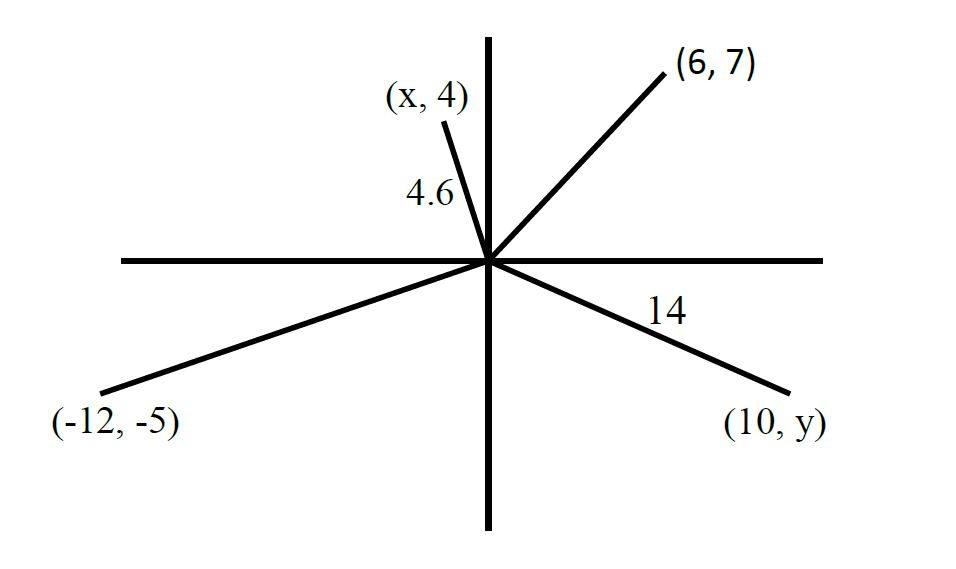
\includegraphics[height=1in]{160H11pic1.jpg}~
 
\end{image}

Quadrant I:
$$\answer[tolerance=0.1]{49.4}\mbox{ degrees}$$

Quadrant II:
$$\answer[tolerance=0.1]{119.6}\mbox{ degrees}$$

Quadrant III:
$$\answer[tolerance=0.1]{202.6}\mbox{ degrees}$$

Quadrant IV:
$$\answer[tolerance=0.1]{315.6}\mbox{ degrees}$$
\end{problem}
 
 
 
 
 
  \section{Lecture 30}
  \begin{problem}\label{prob:160hom12prob1}
  Find $x$.  Round your answers to one decimal place.
\begin{image}
   
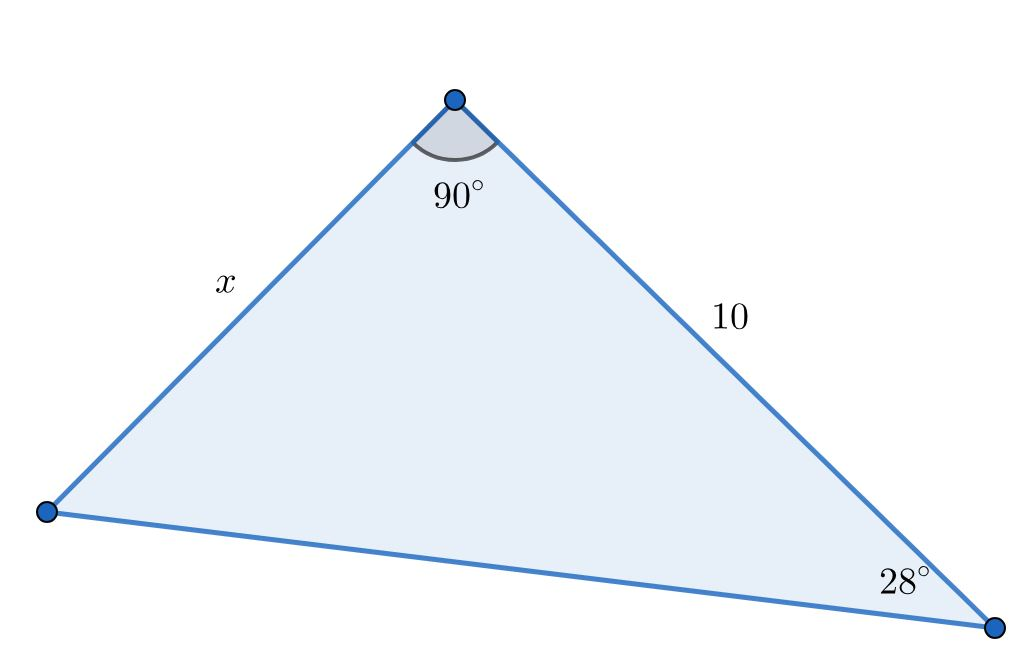
\includegraphics[height=1in]{160H12pic1.jpg}~
 
\end{image}
$$x=\answer[tolerance=0.1]{5.3}$$
\end{problem}

\begin{problem}\label{prob:160hom12prob2}
Find $x$.
\begin{image}
   
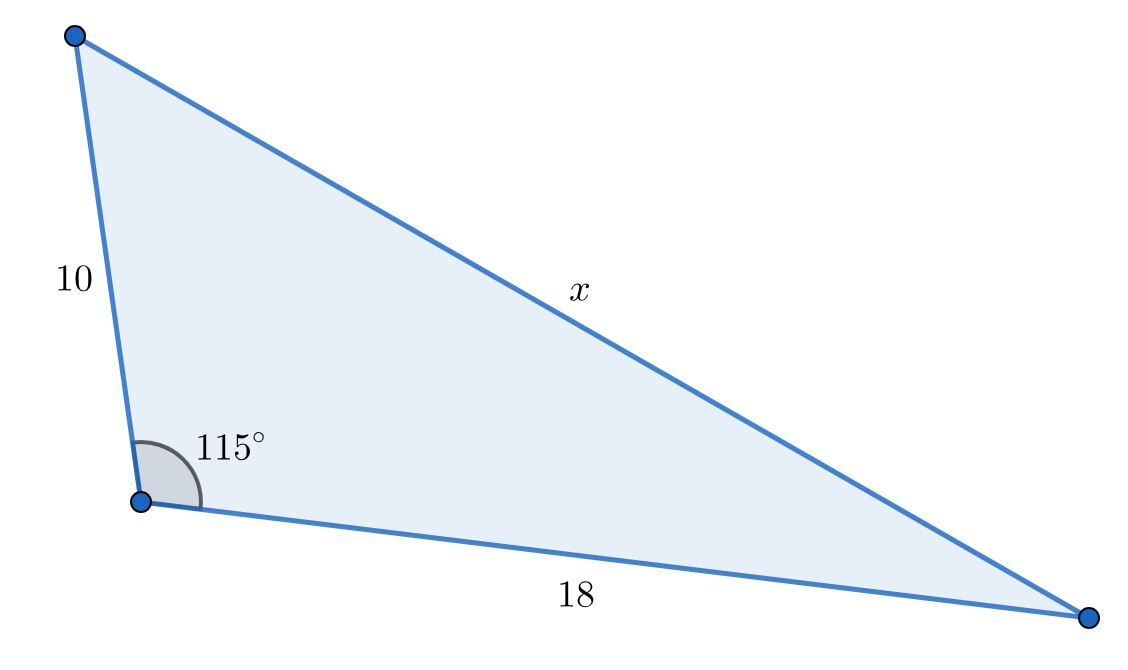
\includegraphics[height=1in]{160H12pic3.jpg}~
 
\end{image}
$$x=\answer[tolerance=0.1]{24}$$
\end{problem}

\begin{problem}\label{prob:160hom12prob3}
Find $x$.
\begin{image}
   
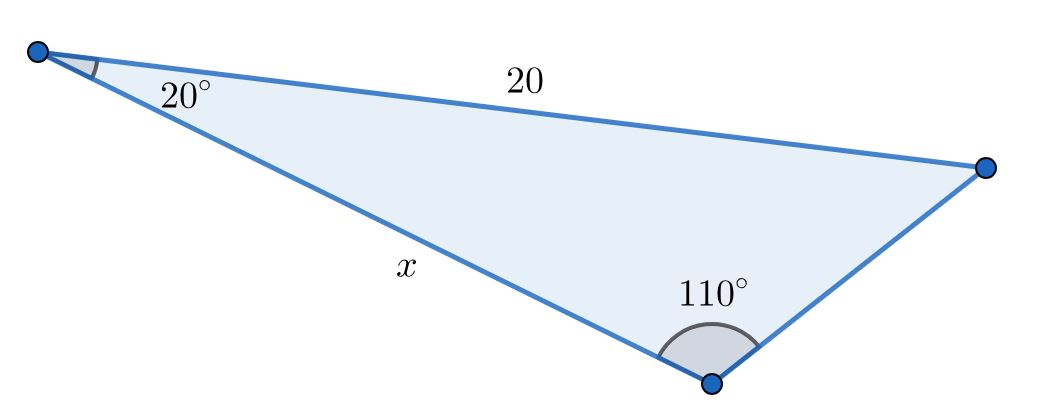
\includegraphics[height=1in]{160H12pic2.jpg}~
 
\end{image}
$$x=\answer[tolerance=0.1]{16.3}$$
\end{problem}


\end{document} 